\documentclass[aspectratio=169]{beamer}

\mode<presentation>
{
  \usetheme{default}
  \usecolortheme{default}
  \usefonttheme{default}
  \setbeamertemplate{navigation symbols}{}
  \setbeamertemplate{caption}[numbered]
  \setbeamertemplate{footline}[frame number]  % or "page number"
  \setbeamercolor{frametitle}{fg=white}
  \setbeamercolor{footline}{fg=black}
} 

\usepackage[english]{babel}
\usepackage[utf8x]{inputenc}
\usepackage{tikz}
\usepackage{courier}
\usepackage{array}
\usepackage{bold-extra}
\usepackage{minted}
\usepackage[thicklines]{cancel}

\xdefinecolor{dianablue}{rgb}{0.18,0.24,0.31}
\xdefinecolor{darkblue}{rgb}{0.1,0.1,0.7}
\xdefinecolor{darkgreen}{rgb}{0,0.5,0}
\xdefinecolor{darkgrey}{rgb}{0.35,0.35,0.35}
\xdefinecolor{darkorange}{rgb}{0.8,0.5,0}
\xdefinecolor{darkred}{rgb}{0.7,0,0}
\definecolor{darkgreen}{rgb}{0,0.6,0}
\definecolor{mauve}{rgb}{0.58,0,0.82}

\title[2018-03-28-hsf-serialization]{Overview of Serialization Technologies}
\author{Jim Pivarski}
\institute{Princeton University -- DIANA-HEP}
\date{March 28, 2018}

\begin{document}

\logo{\pgfputat{\pgfxy(0.11, 7.4)}{\pgfbox[right,base]{\tikz{\filldraw[fill=dianablue, draw=none] (0 cm, 0 cm) rectangle (50 cm, 1 cm);}\mbox{\hspace{-8 cm}
\includegraphics[height=1 cm]{princeton-logo-long.png}
\includegraphics[height=1 cm]{diana-hep-logo-long.png}}}}}

\begin{frame}
  \titlepage
\end{frame}

\logo{\pgfputat{\pgfxy(0.11, 7.4)}{\pgfbox[right,base]{\tikz{\filldraw[fill=dianablue, draw=none] (0 cm, 0 cm) rectangle (50 cm, 1 cm);}\mbox{\hspace{-8 cm}
\includegraphics[height=1 cm]{princeton-logo.png}
\includegraphics[height=1 cm]{diana-hep-logo.png}}}}}

% Uncomment these lines for an automatically generated outline.
%\begin{frame}{Outline}
%  \tableofcontents
%\end{frame}

% START START START START START START START START START START START START START

\begin{frame}{45 years of serialization formats in HEP}
\vspace{0.25 cm}
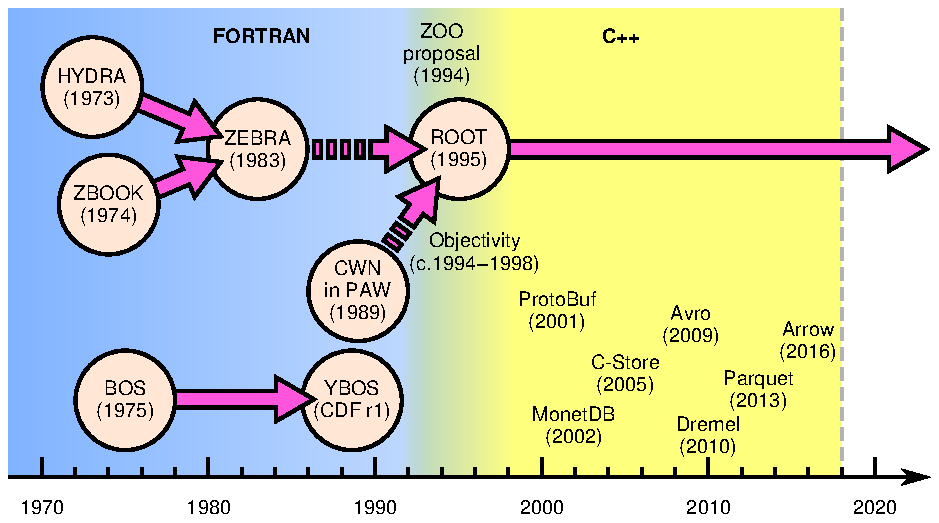
\includegraphics[width=\linewidth]{history.pdf}
\end{frame}

\begin{frame}{Two features have been significant, setting HEP apart}
\vspace{0.5 cm}
\begin{columns}[t]
\column{0.5\linewidth}
\underline{\Large Hierarchically nested structures}

\vspace{0.35 cm}
\textcolor{darkblue}{For example:} event contains jets,

\textcolor{white}{For example:} \hspace{0.5 cm}jets contain tracks,

\textcolor{white}{For example:} \hspace{1 cm}tracks contain hits\ldots

\vspace{0.35 cm}
It's significant that the nested objects have variable size, since structs of structs of integers compile away into constant offsets.

\vspace{0.35 cm}
Fortran (pre-90) didn't have this feature, so physicists had to add it. Now it's much more common.

\column{0.5\linewidth}
\underline{\Large Columnar representation}

\vspace{0.35 cm}
\textcolor{darkblue}{For example:} all values of muon~$p_T$ are contiguous in serialized form, followed by all values of muon~$\eta$, all values of muon~$\phi$, and all \#muons per event.

\vspace{0.35 cm}
Thus, you can read muon~$p_T$ without also reading jet~$p_T$.

\vspace{0.35 cm}
Easy for flat data: just a transpose.

There are several techniques for solving it in general (hot CS topic in early 2000's).
\end{columns}
\end{frame}

\begin{frame}{20 questions}
\vspace{0.15 cm}
\small
\begin{columns}
\column{0.5\linewidth}

\begin{block}{Expressiveness}
\vspace{-0.2 cm}
\begin{itemize}\setlength{\itemsep}{-0.05 cm}
\item Hierarchically nested data or flat tables?
\item Has schema (strongly typed) or dynamic?
\item Schema evolution, if applicable?
\item Language agnostic or specific?
\end{itemize}
\end{block}

\vspace{0.5 cm}

\begin{block}{Performance}
\vspace{-0.2 cm}
\begin{itemize}\setlength{\itemsep}{-0.05 cm}
\item Rowwise or columnar?
\item Compressed/compressible?
\item Robust against bit errors?
\item Serialized/runtime unity?
\end{itemize}
\end{block}

\column{0.5\linewidth}

\begin{block}{Accessibility}
\vspace{-0.2 cm}
\begin{itemize}\setlength{\itemsep}{-0.05 cm}
\item Human readable, binary, or both?
\item Immutable/append only/full database?
\item Parallel readable?
\item Parallel writable?
\item Read streamable?
\item Write streamable?
\item Random accessible?
\item Database-style indexing?
\item RPC protocol?
\end{itemize}
\end{block}

\vspace{-0.2 cm}

\begin{block}{Community}
\vspace{-0.2 cm}
\begin{itemize}\setlength{\itemsep}{-0.05 cm}
\item Has specification?
\item Independent implementations?
\item Size of user base?
\end{itemize}
\end{block}

\end{columns}
\end{frame}


\end{document}
